\chapter{Detector Design and Construction Organization}
\label{vl:tc-overview}

The design and construction of the \dword{dune} detector elements is 
carried out by the international \dword{dune} Project.  \dword{dune}
Collaboration management is responsible for overseeing this portion 
of the global project and ensuring its successful execution.  
The high-level dword{dune} management team consisting of the 
co-spokespersons, \dword{tcoord}, and \dword{rcoord} is responsible 
for the day-to-day administration of the project.  

\section{DUNE Work Flow}
\label{sec:workflow}

Figure~\ref{fig:DUNE_workflow} indicates the time-sequenced set of 
activities needed to implement the \dword{dune} far detector modules.
The \dword{dune} project has direct responsibility for the design, 
prototyping, fabrication, and transportation of the far detector 
elements.  These activities are managed by the \dword{dune} \dword{tc} 
organization under the direction of the \dword{tcoord}.  Activities at 
or in the vicinity of SURF are managed by the on-site integration and
installation team under the direction of the \dword{ipd} as described 
in Chapter~\label{ch:tc-jpo}.  These activities include the receipt,
processing, installation, and operation of the detector components.            
\begin{dunefigure}[\dword{dune} work flow]{fig:DUNE_workflow}
  {\dword{dune} work flow.}
  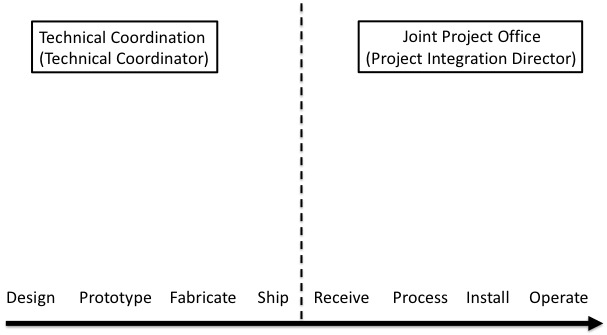
\includegraphics[width=0.99\textwidth]{DUNE_workflow}
\end{dunefigure}

Although responsibilities for the two sets of time-ordered activities 
are clearly delineated, both management teams have roles in supporting
the activities that do not fall under their direct responsibility.  The 
integration and installation team interacts directly with the \dword{dune} 
project team through detector design, prototyping, and construction to 
ensure that fabricated detector elements are properly integrated within 
the supporting infrastructure.  Conversely, the \dword{dune} project 
supports the integration and installation activies at SURF by providing 
some of the dedicated resources (both personnel and equipment) necessary 
for carrying out these activities.  Ensuring proper installation and 
commissioning of the detector elements remains a \dword{dune} project
responsibility even while the global coordination of integration and 
installation activities is managed through the on-site organization.  

The \dword{dune} project has already completed an initial round of design 
and prototyping activities culminating in the construction and operation 
of the \dword{protodune} detectors.  Moving forward, the project is 
updating detector component designs to account for lessons-learned from 
the \dword{protodune} experience.  Upon finalization of the designs, the 
project will construct first production versions of all components, which 
will be installed and operated in a second phase of \dword{protodune} 
operations prior to the start of full-scale production.  The operation 
of the \dword{protodune2} detectors will follow roughly two years after
the end of operations for the corresponding \dword{protodune} detectors.
In a few cases, the production of long lead-time components will need to 
be started in parallel with the operation of first production components 
in \dword{protodune2}.

\section{DUNE Consortia}
\label{sec:consortia}

Construction of the \dword{dune} far \dwords{detmodule} is carried out by 
``consortia of collaboration institutions'' who assume responsibility for 
detector subsystems.  Each consortium plans and executes the construction, 
installation and commissioning of its subsystem.

Management of the consortia is through an overall Consortium Leader and 
a Technical Lead.  The Consortium Leader chairs an institutional board 
composed of one representative from each of the collaboration institutes 
contributing to the activities of the consortium.  Major consortia decisions 
such as technology selections and assignment of responsibilities within 
the institutions are expected to be passed through its Institutional Board.  
These decisions are then passed as recommendation to the \dword{dune} 
\dword{exb}, as described in greater detail below, for formal collaboration 
approval.

Figure~\ref{fig:DUNE_consortia_org} shows an example consortia organizational 
chart with the different parts of the internal consortia structure mandated 
by \dword{dune} Collaboration management.  In addition to the pieces described 
above, the consortium in most cases needs to manage sub-system deliverables 
that are supported by more than a single funding agency.  In the example case 
illustrated here, responsibilities for sub-system deliverables are shared 
between the United States, United Kingdom, and Switzerland, where each of the 
funding agencies is expected to manage their own internal projects which have
direct responsibility for their assigned deliverables.  To ensure coordination
between the separate internal projects contributing to the consortium, the 
Technical Lead is responsible for chairing a consortium Project Management 
Board incorporating the separate managers from each of the internal projects.   
\begin{dunefigure}[\dword{dune} Internal Consortia Structure]{fig:DUNE_consortia_org}
  {\dword{dune} Internal Consortia Structure}
  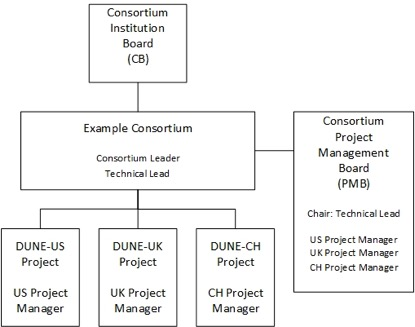
\includegraphics[width=0.99\textwidth]{DUNE_consortia_org}
\end{dunefigure}

In addition to the mandated organizational pieces described here, the consortia 
incorporate additional internal structures as needed to deliver their assigned 
sub-systems.  For example, working groups with convenors are typically appointed 
to focus on specific consortia activities, and steering committees are in many 
cases formed to help guide technical and strategic decisions within the consortia.
Each consortia is also expected to appoint both safety and quality assurance  
representatives as well as a representative with responsibility for integration 
and installation issues.  These individuals are charged with interacting directly 
with appropriate project management team personnel to ensure proper coordination 
on these topics across the consortia.        

\section{DUNE Collaboration Management}
\label{sec:dune_mgmt}

The high-level \dword{dune} collaboration management structure is shown 
in Figure~\ref{fig:DUNE_org}.  The \dword{dune} \dword{exb} is the primary
collaboration decision-making body and as such includes representatives from 
all major areas of activity within the collaboration.
\begin{dunefigure}[\dword{dune} org chart]{fig:DUNE_org}
  {\dword{dune} Organizational Chart}
  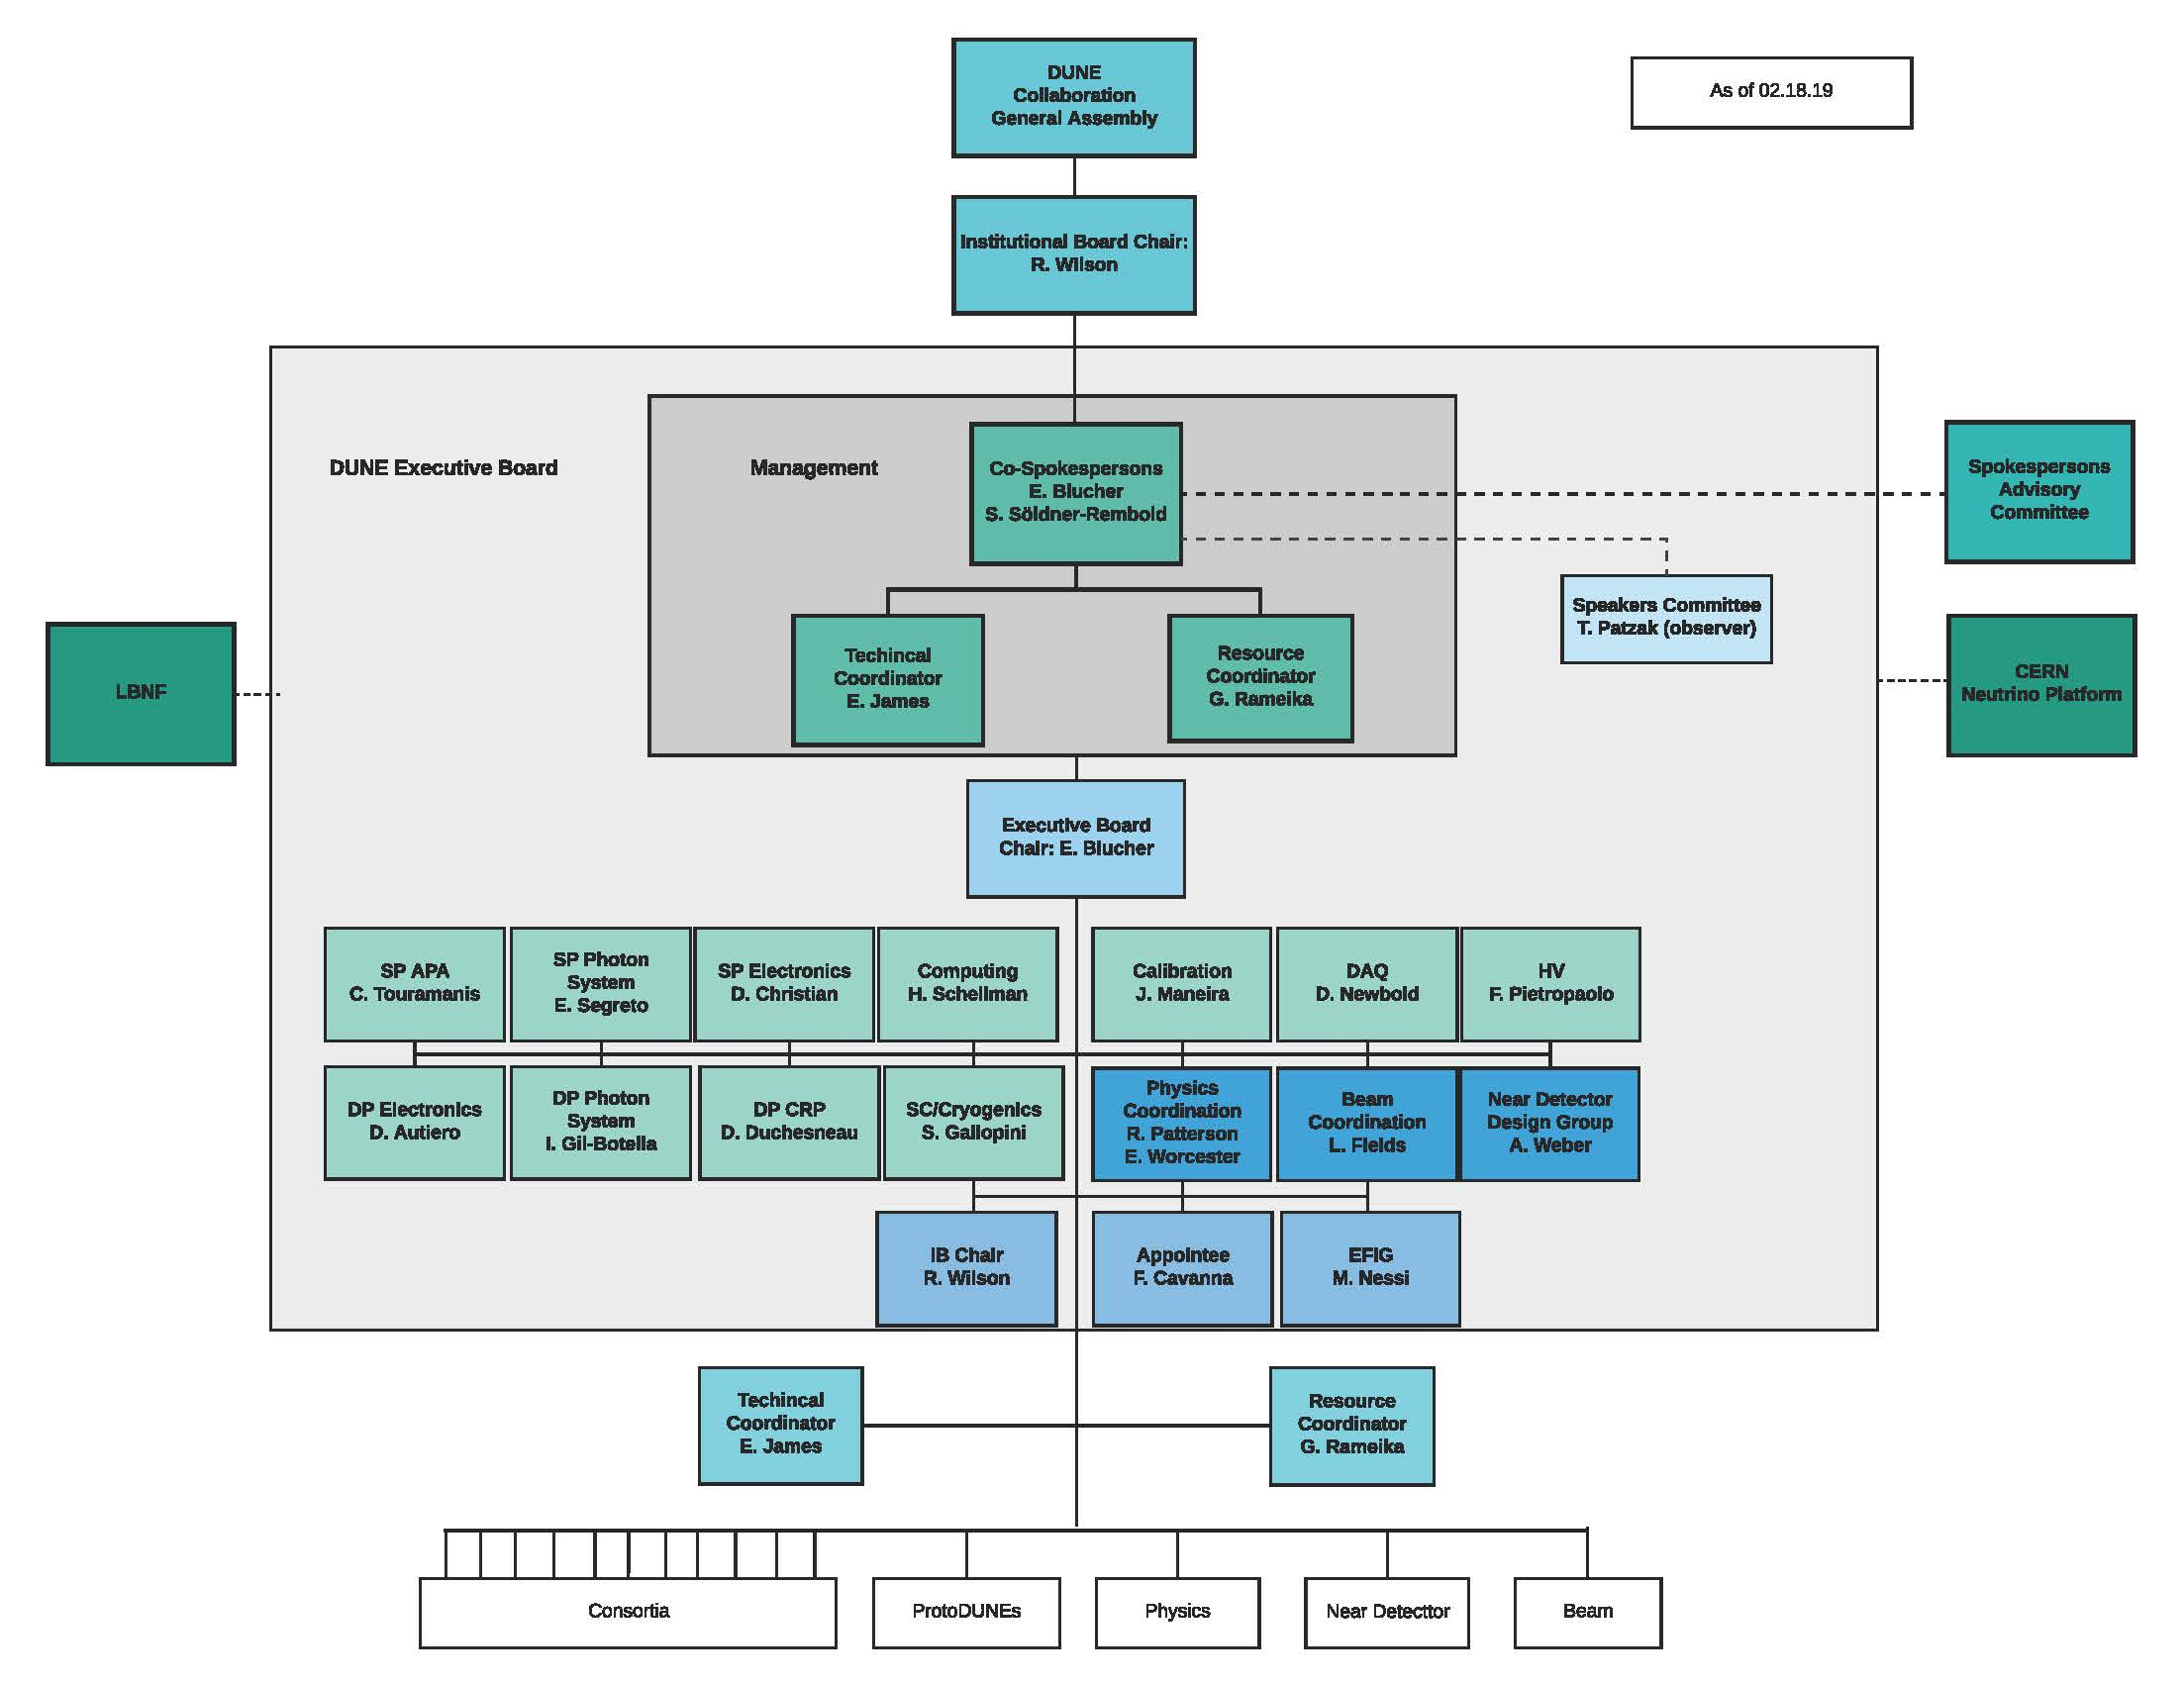
\includegraphics[width=0.99\textwidth]{DUNE_COllab_Mgmt}
\end{dunefigure}

Each of the consortia is represented on the \dword{dune} \dword{exb} by its 
consortium leader.  All collaboration decisions, especially those with potential 
impacts on the \dword{dune} scientific program or connected with the assignment 
of institutional responsibilities, pass through the \dword{exb}.  \dword{exb} 
decisions are expected to be achieved through consensus.  In cases where consensus 
cannot be obtained, decision-making responsibility passes to the co-spokespersons.

\section{\dword{tc}}
\label{sec:tc}

Because the consortia operate as self-managed entities, a strong
\dword{tc} organization is required to ensure overall integration of
the detector elements and successful execution of the detector
construction project.  \dword{tc} areas of responsibility include project
oversight, systems engineering, quality assurance and safety.
\dword{tc} provides support to the \dword{jpo} (see
Section~\ref{sec:pm}) for planning and executing the required detector
integration and installation activities in the nearby surface
facilities and underground detector caverns at \surf.

\dword{tc} is headed by the \dword{tcoord}, who is an \dword{fnal}
employee and is appointed jointly by the \dword{fnal} director and the
\dword{dune} co-spokespersons.  A deputy technical coordinator is
selected from within the collaboration to assist the \dword{tc} in
carrying out their responsibilities.

The \dword{tc} organization supports the work of the consortia and
takes responsibility for integration of the detector
subsystems.  The organization includes teams focusing on project
coordination, detector integration and installation support.  The
project coordination team is led by a lead project controls
specialist, a \dword{qa} manager and an \dword{esh} manager.  The
detector integration team is directed by a lead mechanical and lead
electrical engineer, and inorporates an online computing coordinator.
The installation support team is headed by the coordinators for
activities associated with the integration of detector components on
the surface and installation of components in the underground areas.
Each of the three teams incorporates additional personnel that support
these individuals in carrying out their areas of responsibility.
Figure~\ref{fig:DUNE_tc} shows the \dword{dune} \dword{tc} organizational chart.
\begin{dunefigure}[\dword{dune} \dword{tc} org chart]{fig:DUNE_tc}
  {\dword{dune} \dword{tc} Organizational Chart}
  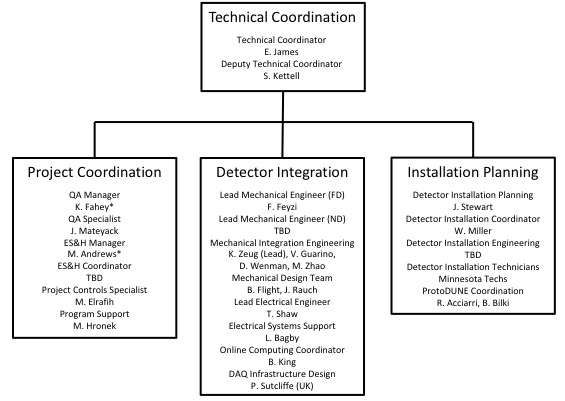
\includegraphics[width=0.99\textwidth]{DUNE_tc}
\end{dunefigure}

\Dword{tc} is led by the \dword{tcoord}, who runs the \dword{tb} that
reviews \dword{dune} technical options. The \dword{tc} organizational
chart is shown in Fig.~\ref{fig:TC_org_chart}.
\begin{dunefigure}[\dword{tc} organizational chart]{fig:TC_org_chart}
  {\dword{dune} \dword{tc} organizational chart.}
  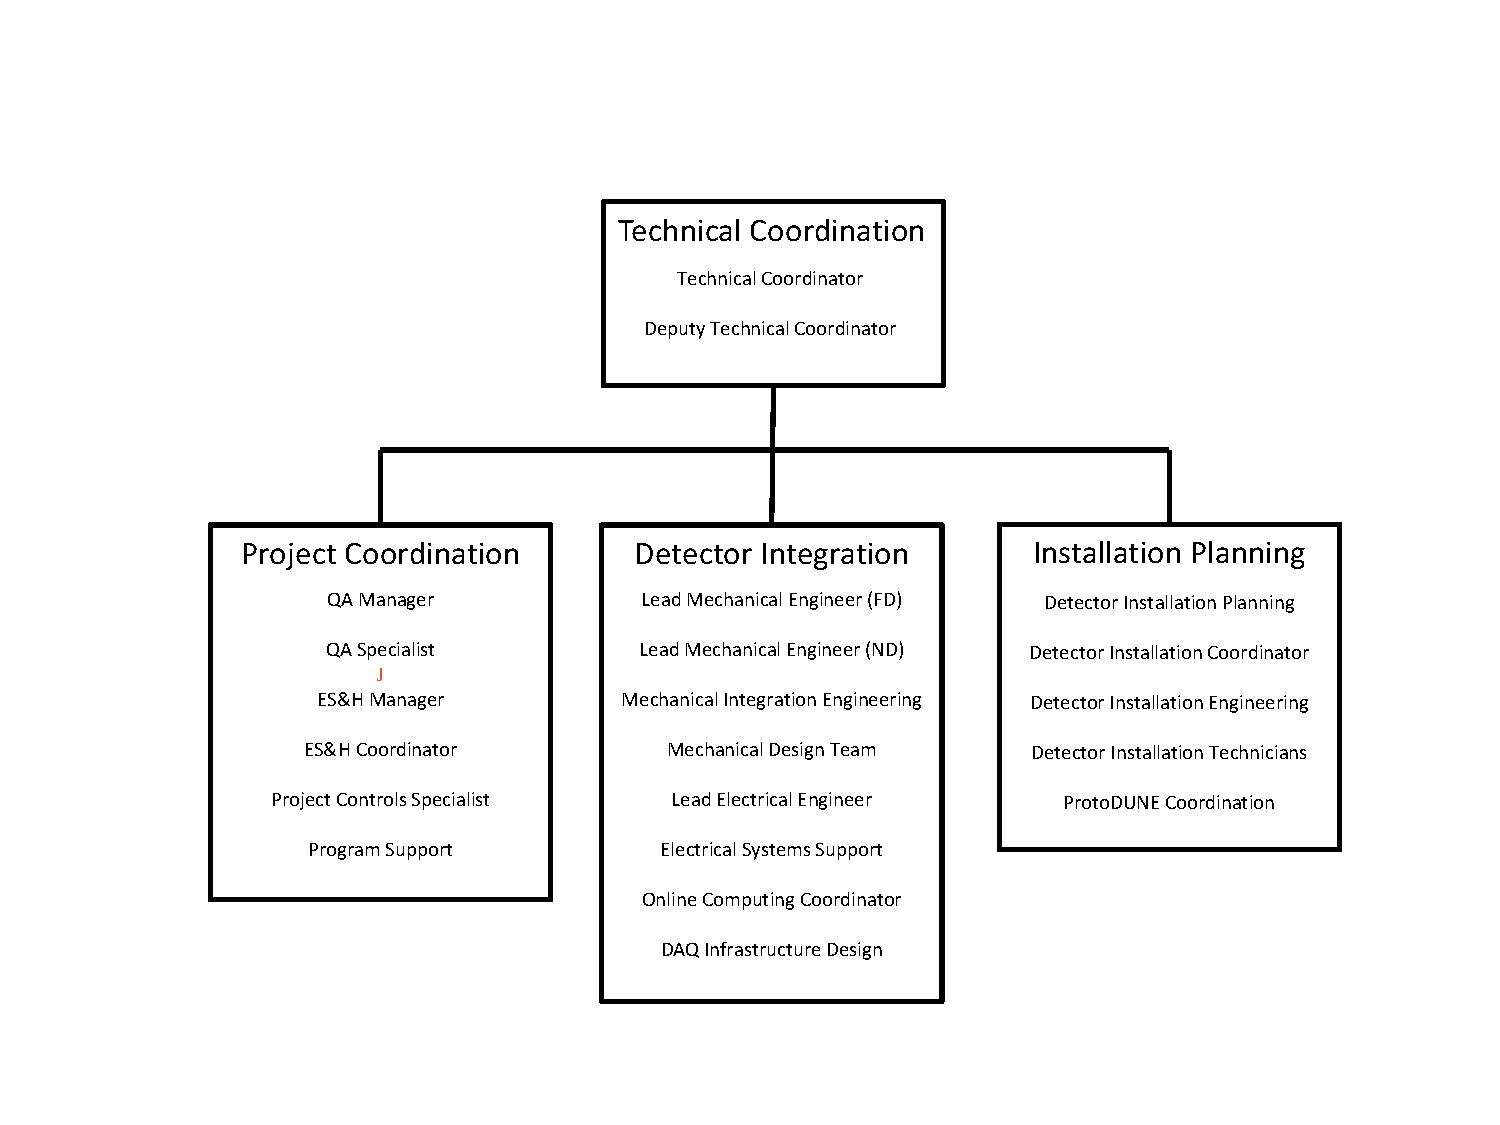
\includegraphics[width=0.99\textwidth]{TC_org_chart}
\end{dunefigure}

\section{DUNE Project Functions}
\label{sec:pm_functions}


\subsection{Safety}
\subsection{Engineering Integration (CAD Models, Drawings, Interfaces, Mechanical \& Electrical)}
\subsection{Change Control and Document Management (Requirements, Quality Assurance Database)}
\subsection{Schedule and Milestones}
\subsection{Partner Agreements and Financial Reporting}

\section{DUNE Project Management}
\label{sec:pm}


\fixme{I'm not clear on the distinction between board meetings:
  consortium board meetings with all consortium leads? Then tech board
  meetings are at a higher level? Who is involved? Then PMBs with
  funding agencies (since they are responsible for managing their
  projects?}

The \dword{tcoord} manages the overall detector construction project
through regular Technical Board meetings with the consortia leadership
teams and members of the \dword{tc} organization.  These board
meetings provide the primary forums for required interactions between
the consortia leadership teams.

Technical Board meetings are used to evaluate consortia design
decisions with potential impacts on overall detector performance,
ensure that interfaces between the different subsystems are well
understood and documented, and monitor the overall construction
project to identify and address both technical and interface issues as
they arise.

Project board meetings are used to ensure that the scopes of each
consortium are fully documented with assigned institutional
responsibilities, develop and manage risks held within a global
project registry, review and manage project change requests, and
monitor the status of the overall detector construction schedule.

Any decisions generated through these board meetings are passed to the
\dword{dune} \dword{exb} as recommendations for formal approval.
Depending on the specific agenda items for a meeting, the
\dword{tcoord} will invite additional members of the collaboration
with specific knowledge or particular expertise to participate.  In
addition, for major decisions, the \dword{tcoord} will officially
appoint three internal collaboration referees with no direct conflicts
of interest to engage in the process.
